\documentclass[tikz,border=3mm]{standalone}
\usetikzlibrary{decorations.pathmorphing}
\usepgfmodule{nonlineartransformations}
\makeatletter
\def\nltrafo{%
\pgfmathsetmacro{\myx}{\pgf@x+7*sin(\pgf@x*4)}%
\pgf@x=\myx pt}
\makeatother
\begin{document}  
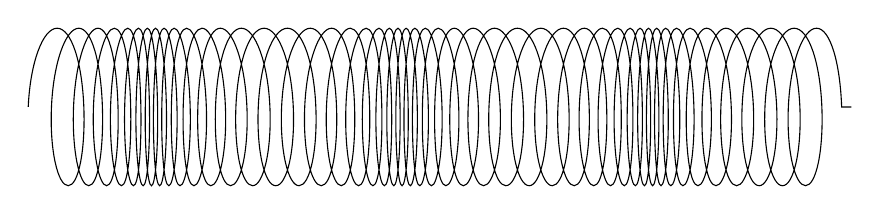
\begin{tikzpicture}
\begin{scope}[transform shape nonlinear=true]
 \pgftransformnonlinear{\nltrafo}
 \draw[decorate, decoration={coil,aspect=0.2, segment length=2mm, amplitude=10mm}]
 (0,0) --(10,0);

\end{scope}
\end{tikzpicture}
\end{document}